\section*{Q3: Temporal Difference}
\subsection*{1}

SARSA was chosen. SARSA is on policy meaning that the current
policy will be updated and hence is generally "safer" meaning 
more reliable updating. Furthermore, on-policy can be argued to 
be better in this scenario given that it's not advantageous to
explore policies that result in the incorrect absorbing states
or into a wall. 

For SARSA to converge to the optimal value function, the policies
need to be a GLIE sequence and the step sizes of $\alpha$ must be 
Robbins-Munro. The default value for $a_t$ is $\frac{1}{t+1}$ which 
satisfies the Robbins-Munro condition (this can be substituted in 
for a different policies for $a_t$ for comparison).

Similar to Monte Carlo, a large number of episodes are sampled 
to be GLIE. Here the default is $5000$ which should provide 
sufficient coverage. 

The Q here is initialised to be random values (Q can be 
set arbitrarily). 
For SARSA, the initialisation of Q also needs
to have the behaviour that at the absorbing states 
$Q[end, \cdot] = 0$. The game does not
provide the absorbing states, so before the Q is updated 
the next state $s'$ is checked to determine if it is an absorbing
state. If $s'$ is an absorbing state then the $Q[s', \cdot] = 0$
so the update becomes $Q[s, a] = Q[s, a] + \alpha_t [R - Q[s,a]]$.

% TODO

\subsection*{2}

\begin{figure}[H]
    \centering
    \begin{subfigure}[b]{0.4\textwidth}
        \centering
        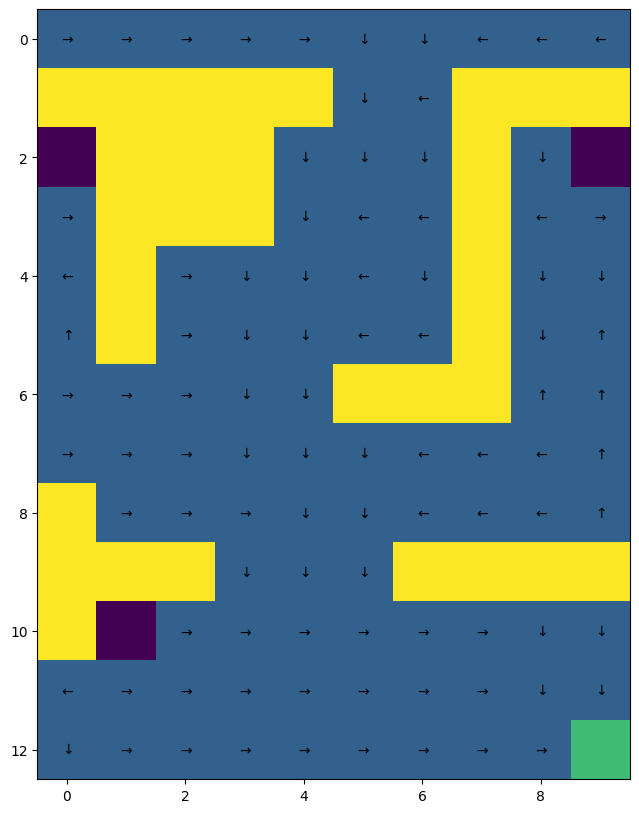
\includegraphics[width=\textwidth]{assets/td/td_policy.png}        
        \caption{Temporal Difference Policy}
    \end{subfigure}
    \hfill 
    \begin{subfigure}[b]{0.4\textwidth}
        \centering
        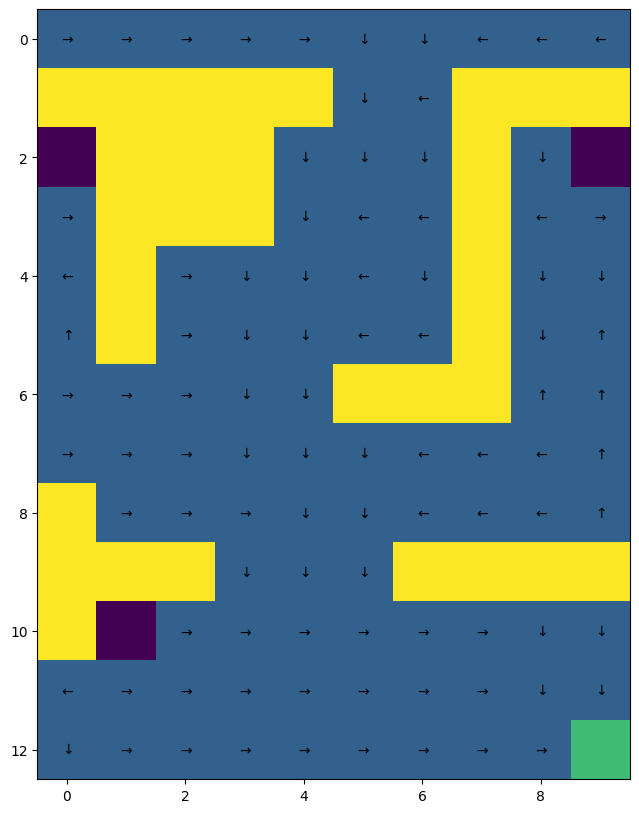
\includegraphics[width=\textwidth]{assets/td/td_policy.png}        
        \caption{Temporal Difference Value Function}
    \end{subfigure}
    \caption*{Graphical Representations of Temporal Difference Results}
\end{figure} 


\subsection*{3}

\begin{figure}[H]
    \centering
    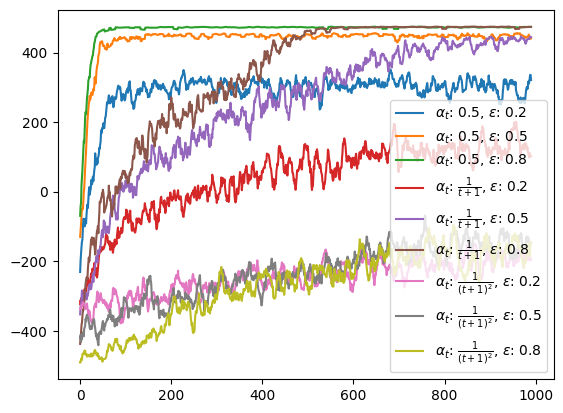
\includegraphics[width=\textwidth]{assets/td/td_analysis.png}        
    \caption{Temporal Difference analysis}
    \label{figure:temporal difference analysis}
\end{figure} 

In figure \ref{figure:temporal difference analysis}, the total reward
overtime is plotted for different configurations of the learning rate
(function for $\alpha_t$) and epsilon. The data smoothed out 
using a moving average make the data more legible.

It can be seen that having a high epsilon results in a faster 
convergence to the optimal policy. This is to be expected as 
low epsilon results in larger explorations of the environment,
whereas higher epsilon is more greedy - taking the current found 
optimal path more frequently. 